\subsubsection{Subsystem Overview}
The computing platform's power subsystem is comprised of batteries, voltage converters, and other supporting circuitry. The devices powered by this system are the:

\begin{itemize}
\item Platform Management Board (Raspberry Pi) -- maximum current draw of 1 A and a typical current draw of 400 mA, and
\item Programmable Logic Board (Zedboard) -- maximum current draw of 4 A and a typical current draw of 1 A
\end{itemize}

The power system must provide continuous power to the computing platform for at least 20 minutes (\textbf{F.PR.1}).

It is important to note that this power system is \textit{distinct} from the multirotor's power supply to avoid noise from the motors interfering with the computing platform. 

\subsubsection{Battery}
The power subsystem utilizes Lithium-ion batteries coupled with a battery management system. In order to
power the computing system for 20 minutes the battery will need to have a capacity of 233mAh, however as that is a non-standard size and to allow for a margin of error an 11.1V battery with a 1000mAh capacity will be used. This should provide 43 minutes of operation.

\subsubsection{Battery Management}
 
The battery management system (seen in Figure \ref{powerdiag}) consists of two DC-DC converters, a battery protection board, and a battery monitor. 

\begin{figure}[H]
\centering
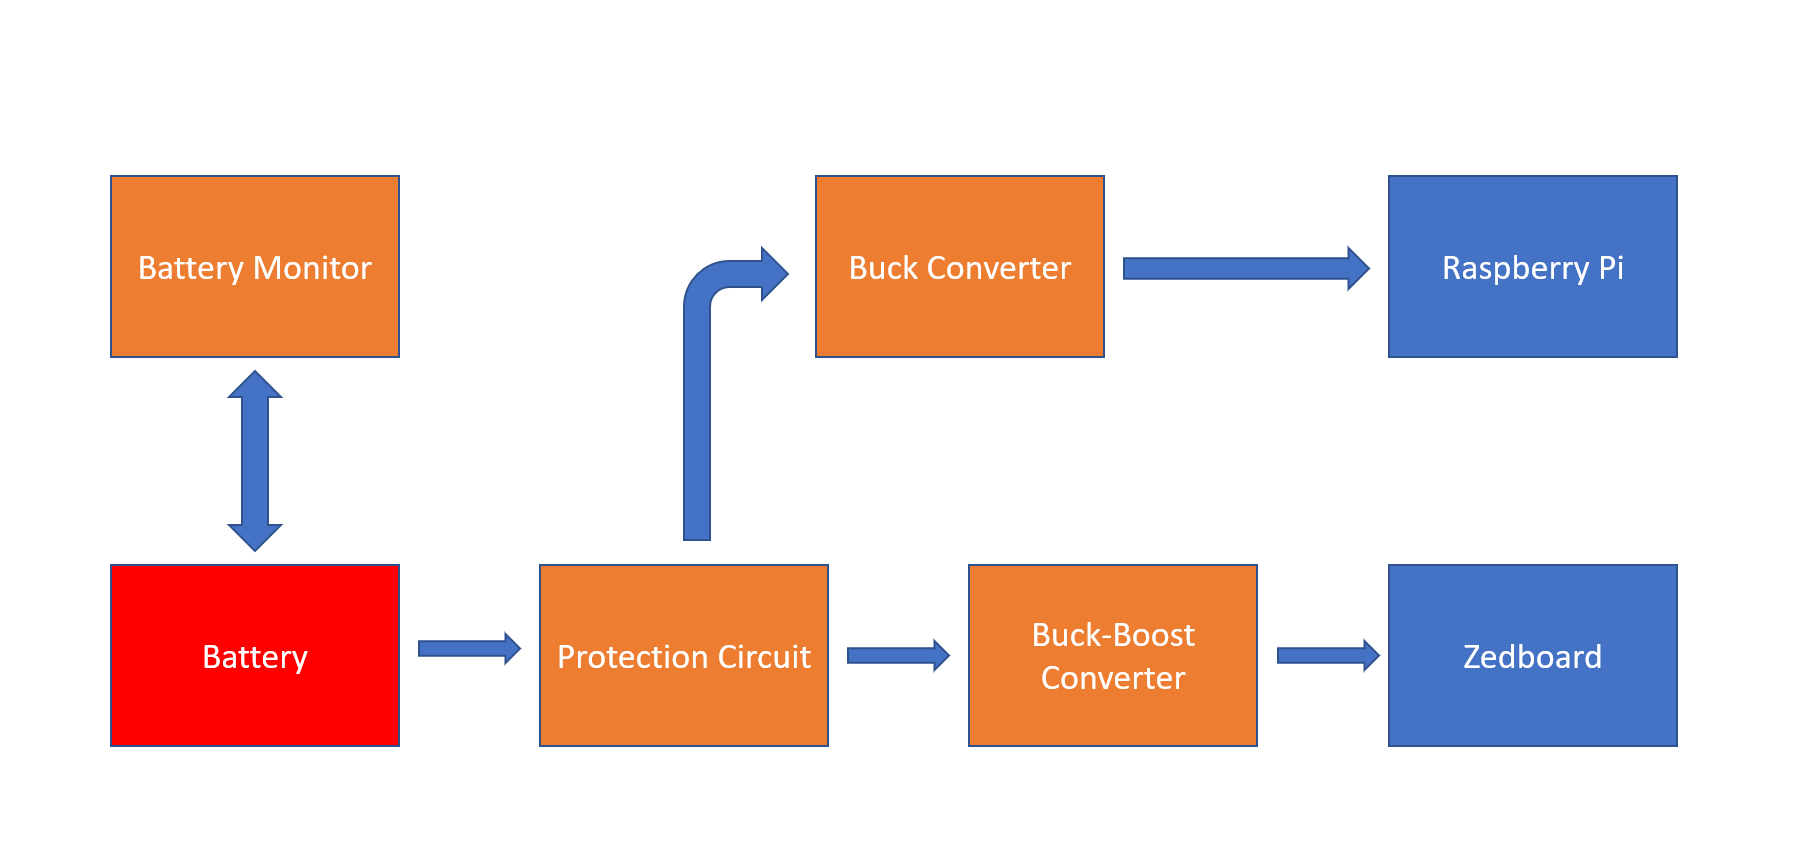
\includegraphics[width=15cm]{img/Power_Diagram.png}
\caption{Computing Platform Power Subsystem}
\label{powerdiag}
\end{figure}

DC-DC conversion is accomplished using a buck converter for the 5 V output and a buck-boost converter for the 12 V output. 

The battery protection board consists of a Zener diode to provide undercurrent protection, a fuse to provide overcurrent protection, and a simple circuit to provide reverse polarity protection (\textbf{F.PR.4-5}). Reverse polarity protection is achieved using connectors that cannot be connected in reverse (\textbf{F.PR.6}). 